\documentclass[12pt]{article}
\usepackage[margin=2.5cm]{geometry}
\usepackage{enumerate}
\usepackage{amsfonts}
\usepackage{amsmath}
\usepackage{fancyhdr}
\usepackage{amsmath}
\usepackage{amssymb}
\usepackage{amsthm}
\usepackage{mdframed}
\usepackage{graphicx}
\usepackage{subcaption}
\usepackage{listings}
\usepackage{xcolor}


\begin{document}
\title{CSC148 Worksheet 1 Review}
\author{Hyungmo Gu}
\maketitle

\section*{Question 1}
\begin{center}
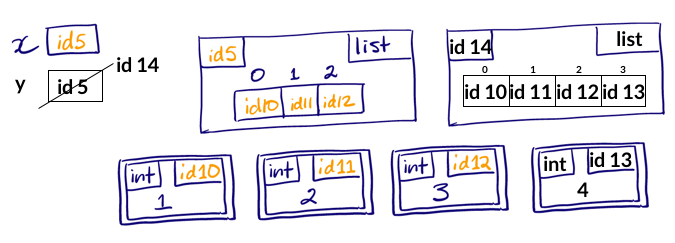
\includegraphics[width=0.8\linewidth]{images/worksheet_1_review_q1_solution.png}
\end{center}

\bigskip

\begin{mdframed}
    \underline{\textbf{Correct Solution:}}

    \bigskip

    \begin{center}
    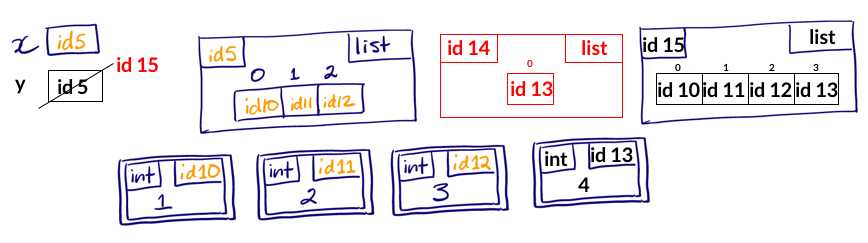
\includegraphics[width=0.8 \linewidth]{images/worksheet_1_review_q1_correction.png}
    \end{center}

\end{mdframed}

\section*{Question 2}
\begin{center}
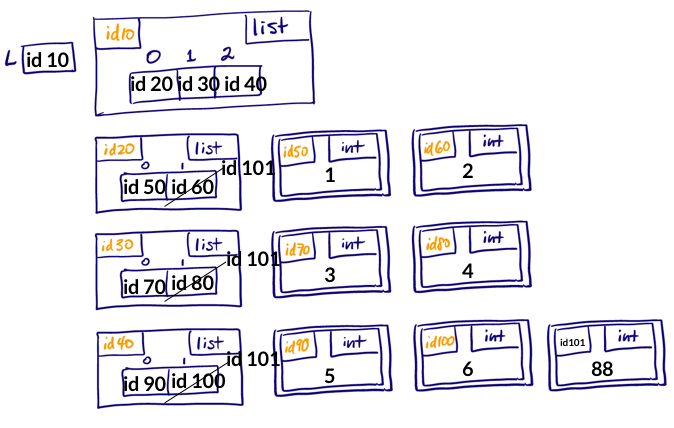
\includegraphics[width=0.8\linewidth]{images/worksheet_1_review_q2_solution.png}
\end{center}


\begin{mdframed}
    \underline{\textbf{Correct Solution:}}

    \bigskip

    \begin{center}
    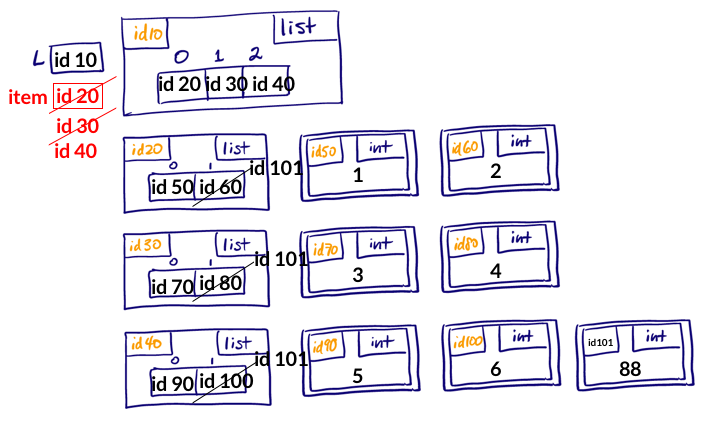
\includegraphics[width=0.8 \linewidth]{images/worksheet_1_review_q2_correction.png}
    \end{center}

\end{mdframed}

\bigskip

\textbf{Notes:}

\begin{itemize}
    \item Learned that `item' in \textbf{for item in L:} is a variable with its
    value changing on every iteration. This is too cool!

    \begin{center}
    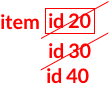
\includegraphics[width=0.2\linewidth]{images/worksheet_1_review_q2_note.png}
    \end{center}
\end{itemize}

\section*{Question 3}
\begin{center}
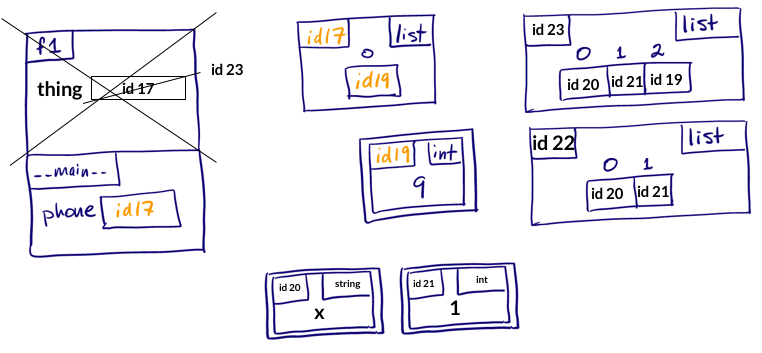
\includegraphics[width=0.8\linewidth]{images/worksheet_1_review_q3_solution.png}
\end{center}

\bigskip


\section*{Question 4}

\end{document}